\documentclass[a4paper,11pt]{article}
%\documentclass[a4paper,11pt,twocolumn]{article}

\usepackage{natbib}
\setlength{\bibsep}{1pt}
%\newcommand{\bibfont}{\footnotesize}

\usepackage{enumitem}

\usepackage[dvips,colorlinks,bookmarksopen,bookmarksnumbered,citecolor=red,urlcolor=red]{hyperref}

\usepackage{moreverb}
\addtolength{\hoffset}{-2cm}
\addtolength{\textwidth}{4cm}
\addtolength{\voffset}{-3cm}
\addtolength{\textheight}{5cm}
\usepackage{array,amsmath,graphicx}
\author{Daniel Reinert}
\title{ICON Documentation: Surface Albedo from MODIS Data}
%\date{ 2007} % optional  
\begin{document}  \maketitle

%-------------------------------------------------------------------------

%\chapter{Physical processes}

\section{Surface albedo}
Albedo is defined as the ratio of upwelling to downwelling radiative flux at the surface. The downwelling flux may be written as the sum of a direct and a diffuse component. Thus, two 
different albedos based on either the diffuse or direct flux component can be defined. White-sky albedo is defined as albedo in the absence of a direct component when the diffuse 
component is isotropic. Black sky albedo is defined as albedo in the absence of a diffuse component. While black sky albedo is a function of the solar zenith angle, white sky albedo 
is essentially zenith angle independent.

Within the shortwave radiation scheme, the reflection at the surface is handled considering both direct and diffuse downward radiation fluxes. For this, spectral albedos for parallel and 
diffuse radiation are needed. The spectral albedos distinguish between the visible ($0.3\,-\,0.7\,\mathrm{\mu m}$) and near-infrared ($0.7\,-\,5.0\,\mathrm{\mu m}$) spectral bands. Thus, 
$4$ albedo values ($\alpha_{\mathrm{dir}}^{vis}$, $\alpha_{\mathrm{dir}}^{nir}$, $\alpha_{\mathrm{diff}}^{vis}$, $\alpha_{\mathrm{diff}}^{nir}$) are required for each grid point. The 
indices $\mathtt{dir}$ and $\mathtt{diff}$ indicate the type of radiation (direct or diffuse), whereas the indices $\mathtt{vis}$ and $\mathtt{nir}$ distinguish the spectral bands 
(UV-visible or near-infrared). In the following we will separately discuss snow-free and snow-covered land, open water, sea-ice and fresh water lake points.


\subsection{Albedo for diffuse downward radiation (white sky)}

\subsubsection{Snow-free land points}
Over snow-free land, white sky surface albedos ($\alpha_{\mathrm{diff}}^{vis}$, $\alpha_{\mathrm{diff}}^{nir}$) are derived from monthly mean climatologies build from 16-days MODIS 
albedo over the year 2000-2003 \citep{Schaaf:2002}. Separate datasets are available for UV-visible and near-infrared spectral bands. The model does a linear interpolation between 
successive months, assuming that the monthly field belongs to the $15\mathrm{th}$ of the month. The values are updated on a daily basis. If land tiles are used, the same MODIS albedo 
is assigned to all land tiles of a single grid cell.


\subsubsection{Snow-covered land points}
The snow albedo for visible and near-infrared spectral bands is calculated by
\begin{align}
 \alpha_{\mathrm{diff}}^{vis} = \alpha_{\mathrm{diff}}^{nir} =\alpha_{s,min} + S_{age}\,\left(\alpha_{s,max} - \alpha_{s,min}\right)\,,
\end{align}
with $\alpha_{s,max}=0.85$ and $\alpha_{s,min}=0.5$. The reduction of snow albedo with increasing snow age is taken into account by an ageing function $0\leq S_{age}\leq 1$. The value 
of $S_{age}$ is $1$ for fresh snow and approaches 0 for old snow. The variation of $S_{age}$ with time consists of a constant ageing and a regeneration by falling snow:
\begin{align}
 \Delta S_{age} = S_{age}\left[\frac{P_{snow}}{P_{norm}} - \frac{\Delta t}{\tau_{a}}\right]
\end{align}
$P_{snow}$ is the snowfall rate, and $P_{norm}=5\,\mathrm{mm}/24\,\mathrm{h}$. If no snow exists, $S_{age}=1$ is prescribed. Note that for needleleaved and broadleaved forests snow 
ageing is not taken into account and the snow albedo is limited to values of about $0.3$.


\subsubsection{Open-water points}
For open-water points, the white sky albedos are set to a constant value.
\begin{align}
  \alpha_{\mathrm{diff}}^{vis} = \alpha_{\mathrm{diff}}^{nir} = 0.07
\end{align}


\subsubsection{Sea-ice points}
The ice surface albedo for diffuse radiation is approximated as:
\begin{align}
  \alpha_{\mathrm{diff}}^{vis} = \alpha_{\mathrm{diff}}^{nir} = \alpha_{i,max} - 
  \left(\alpha_{i,max}-\alpha_{i,min}\right)\exp\left[-C_{\alpha}\left(\frac{T_{f0}-T_{i}}{T_{f0}}\right)\right]\,, \label{eq_icealbedo}
\end{align}
where $\alpha_{i,max}=0.7$ and $\alpha_{i,min}=0.43$ are maximum and minimum values of the sea-ice albedo, $T_{f0}=273.25\,\mathrm{K}$ is the fresh water freezing point, 
$T_{i}$ is the ice surface temperature and $C_{\alpha}=95.6$ is a fitting coefficient. Equation \ref{eq_icealbedo} is meant to implicitly account (in a crude way) for the seasonal 
changes of $\alpha$. The ice albedo is the lower the warmer, and therefore wetter the ice is.


\subsubsection{Fresh water lake points}
For frozen lakes, equation \ref{eq_icealbedo} is used, too. However, the maximum and minimum ice albedo is set to $\alpha_{i,max}=0.6$ and $\alpha_{i,min}=0.1$, respectively. 
If no ice is present, the surface albedo for diffuse radiation is approximated as
\begin{align}
   \alpha_{\mathrm{diff}}^{vis} = \alpha_{\mathrm{diff}}^{nir} =0.07
\end{align}

\subsubsection{Sample plots}
Figure \ref{fig_albvisdif} and \ref{fig_albnirdif} show the white sky surface albedo (UV-visible and near-infrared) for the 1st June 2012 00UTC as it is 
operationally used by ICON for snow-free land points. Note that compared to the original MODIS data, the Saharan albedo has been slightly reduced in order 
to compensate for a model cold bias in that region.
\begin{figure}[ht]
\begin{minipage}[t]{\textwidth}
  \begin{minipage}[t]{0.498\textwidth}
    \center
    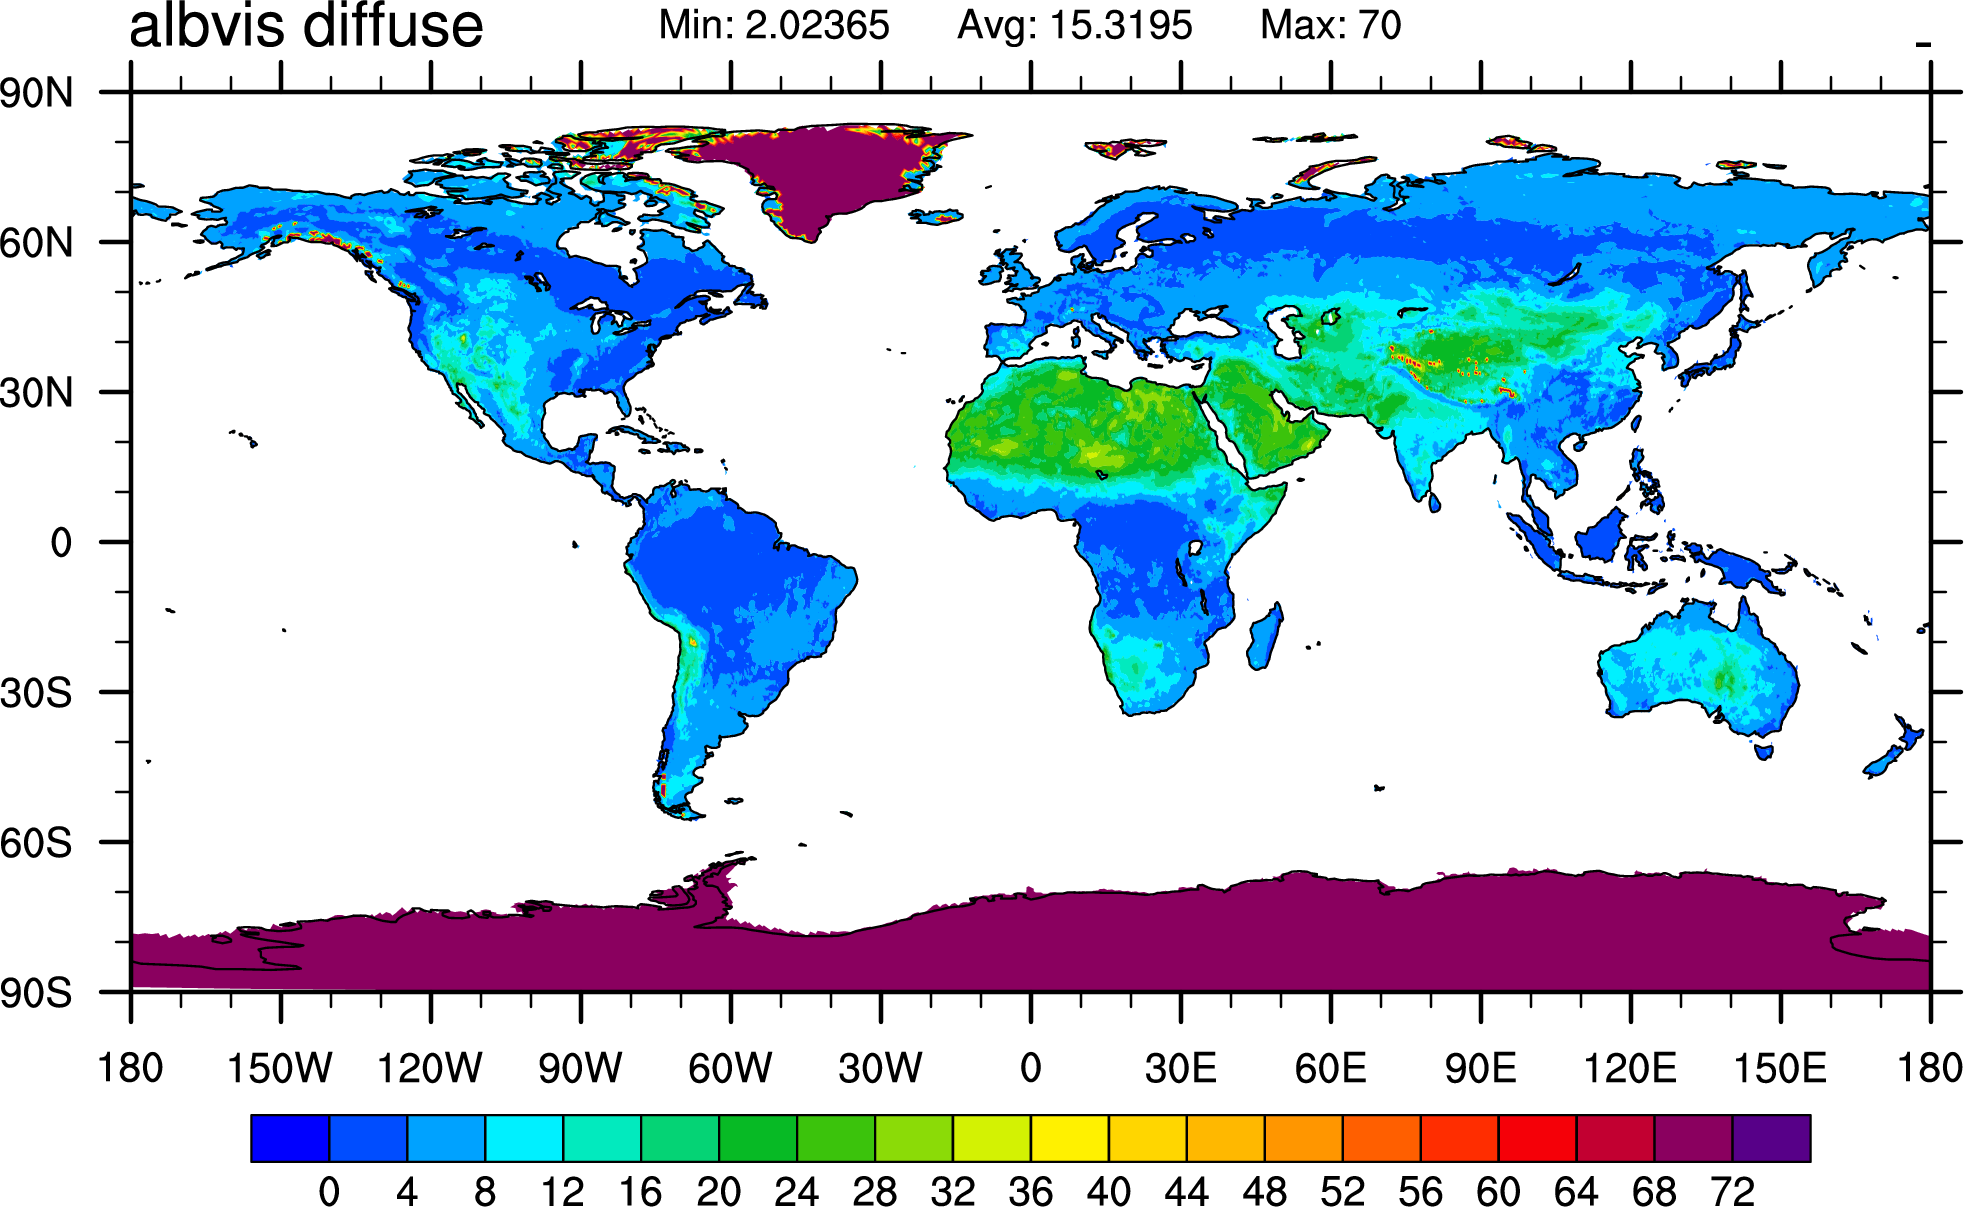
\includegraphics[width=8.1cm]{albvisdif_20120601_tuned.png}
  \end{minipage}
  \begin{minipage}[t]{0.498\textwidth}
    \center
    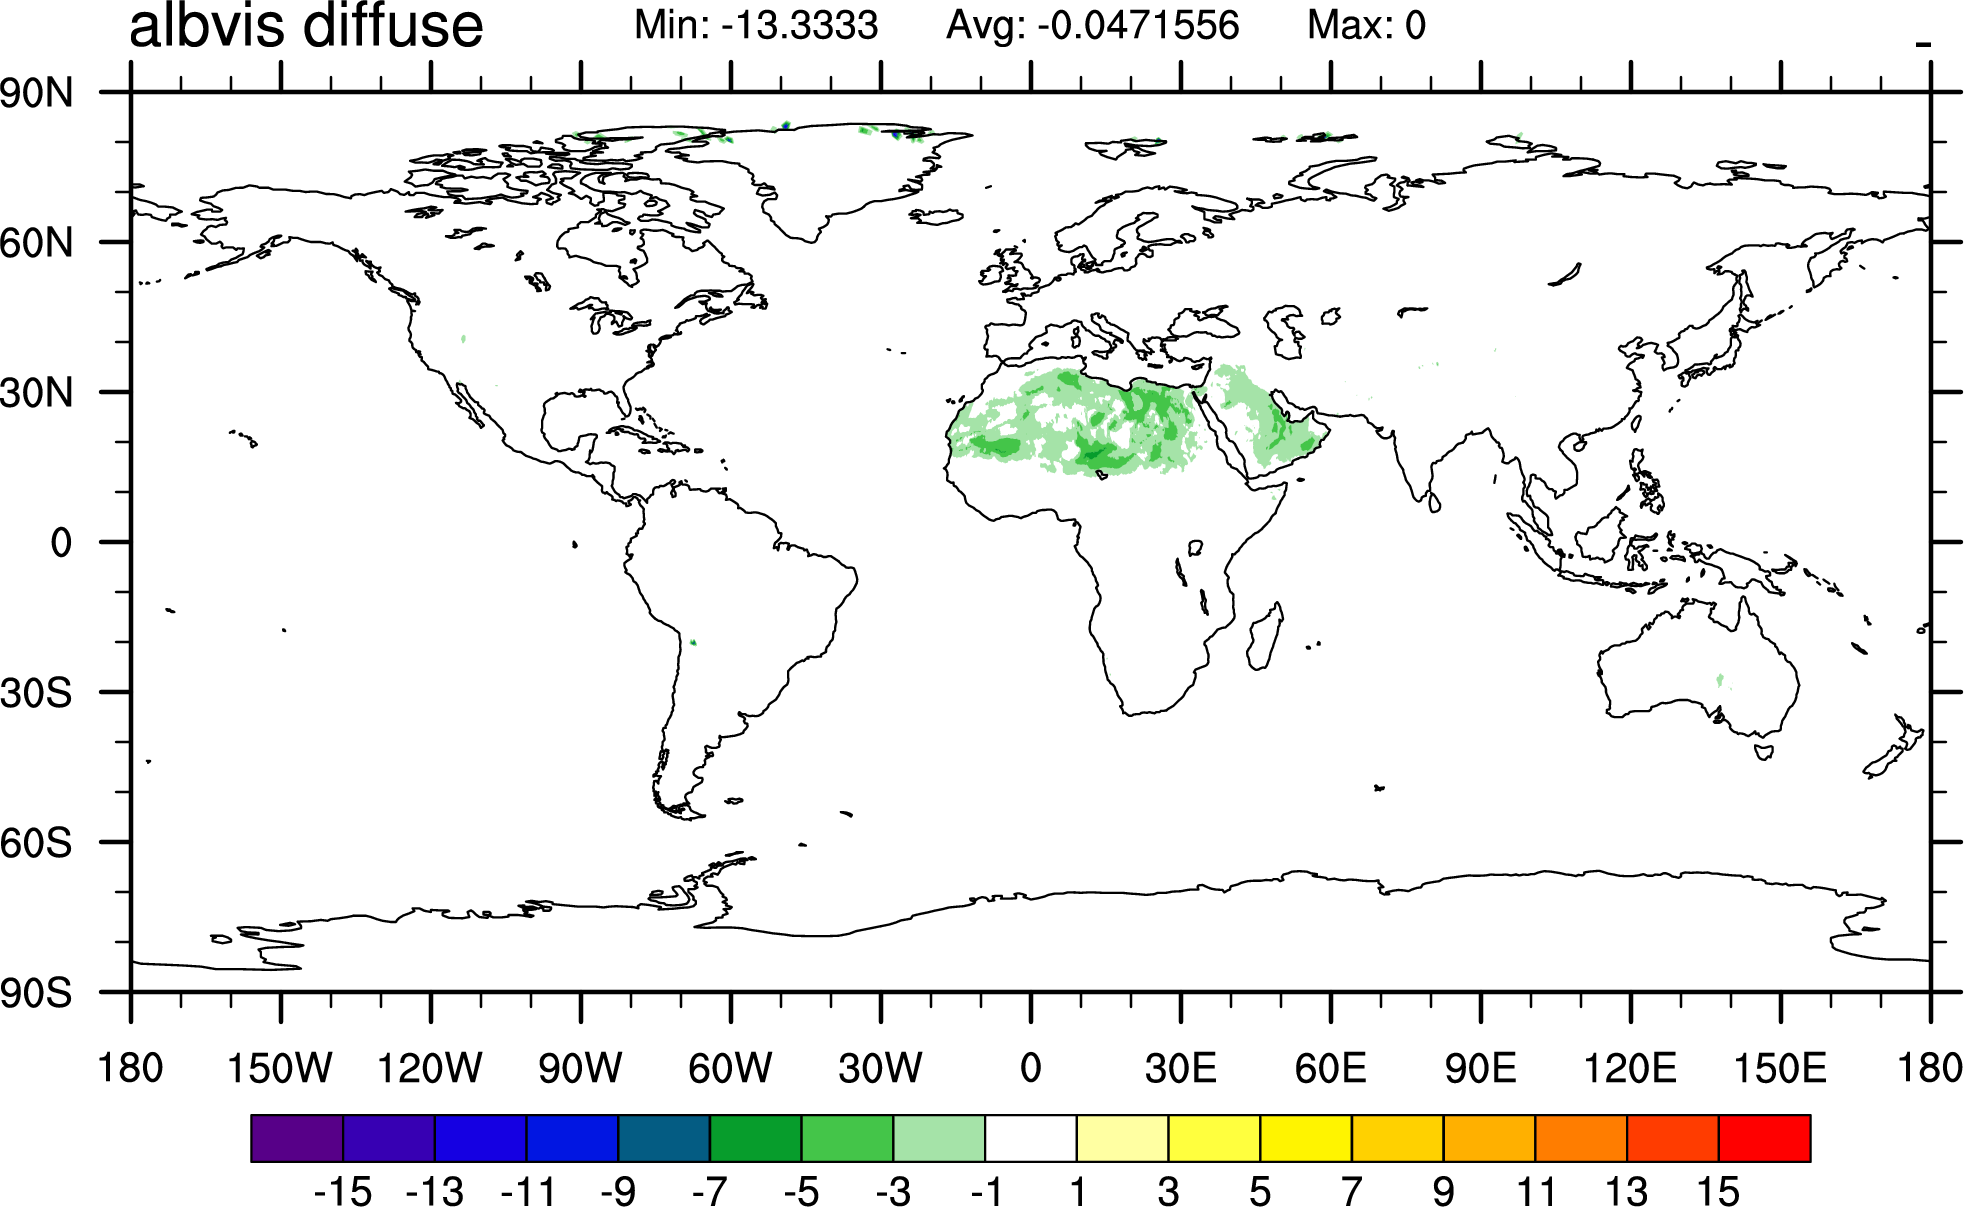
\includegraphics[width=8.1cm]{albvisdif_20120601_tuned-untuned.png}
  \end{minipage}
\end{minipage}
\caption{White sky (diffuse) albedo for UV-visible (left) spectral bands for the 1st June 2012 00UTC and its deviation from the original MODIS values (actual-original).}\label{fig_albvisdif}
\end{figure}

\begin{figure}[ht]
\begin{minipage}[t]{\textwidth}
  \begin{minipage}[t]{0.496\textwidth}
    \center
    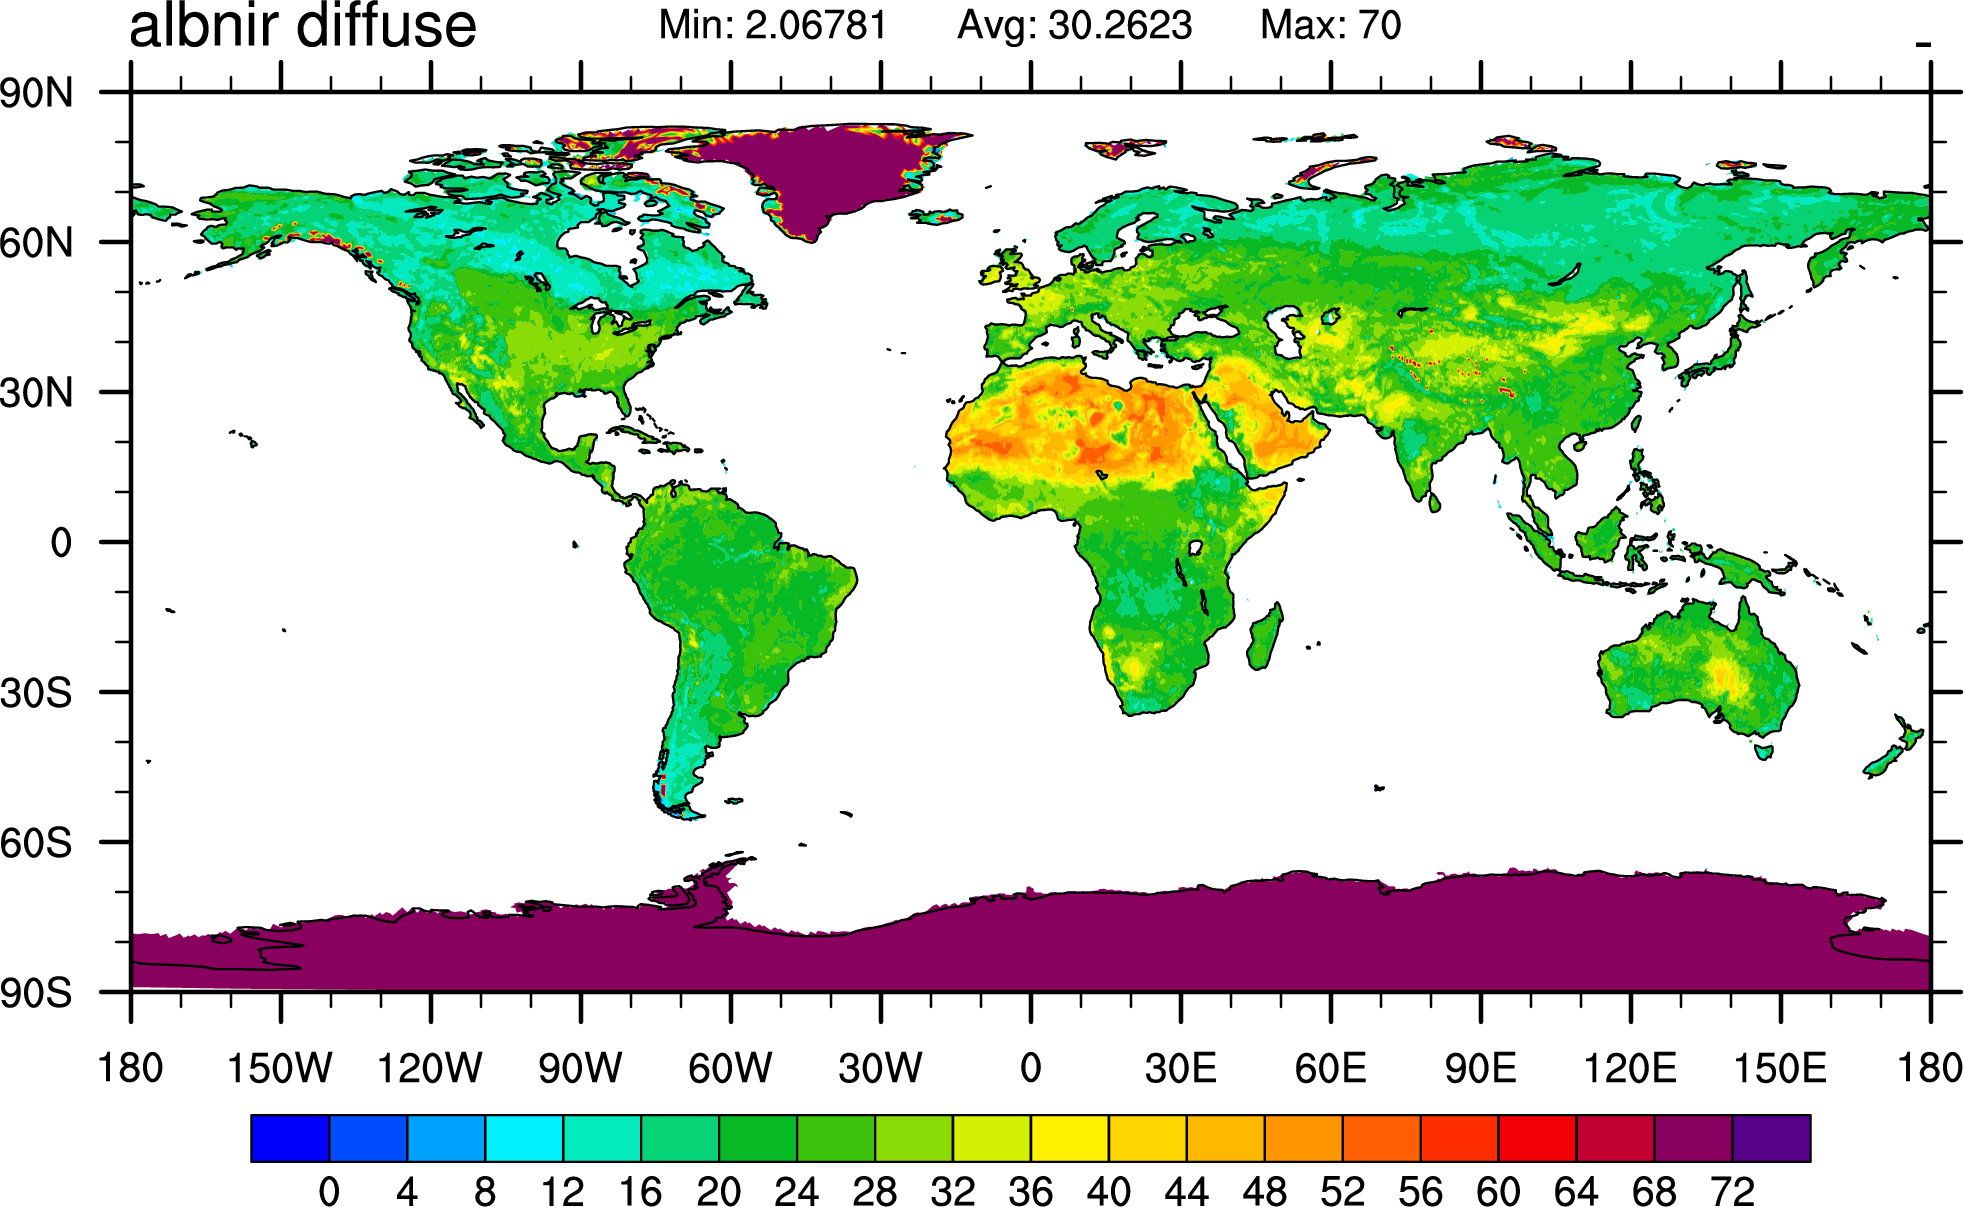
\includegraphics[width=7.7cm]{albnirdif_20120601_tuned.png}
  \end{minipage}
  \begin{minipage}[t]{0.496\textwidth}
    \center
    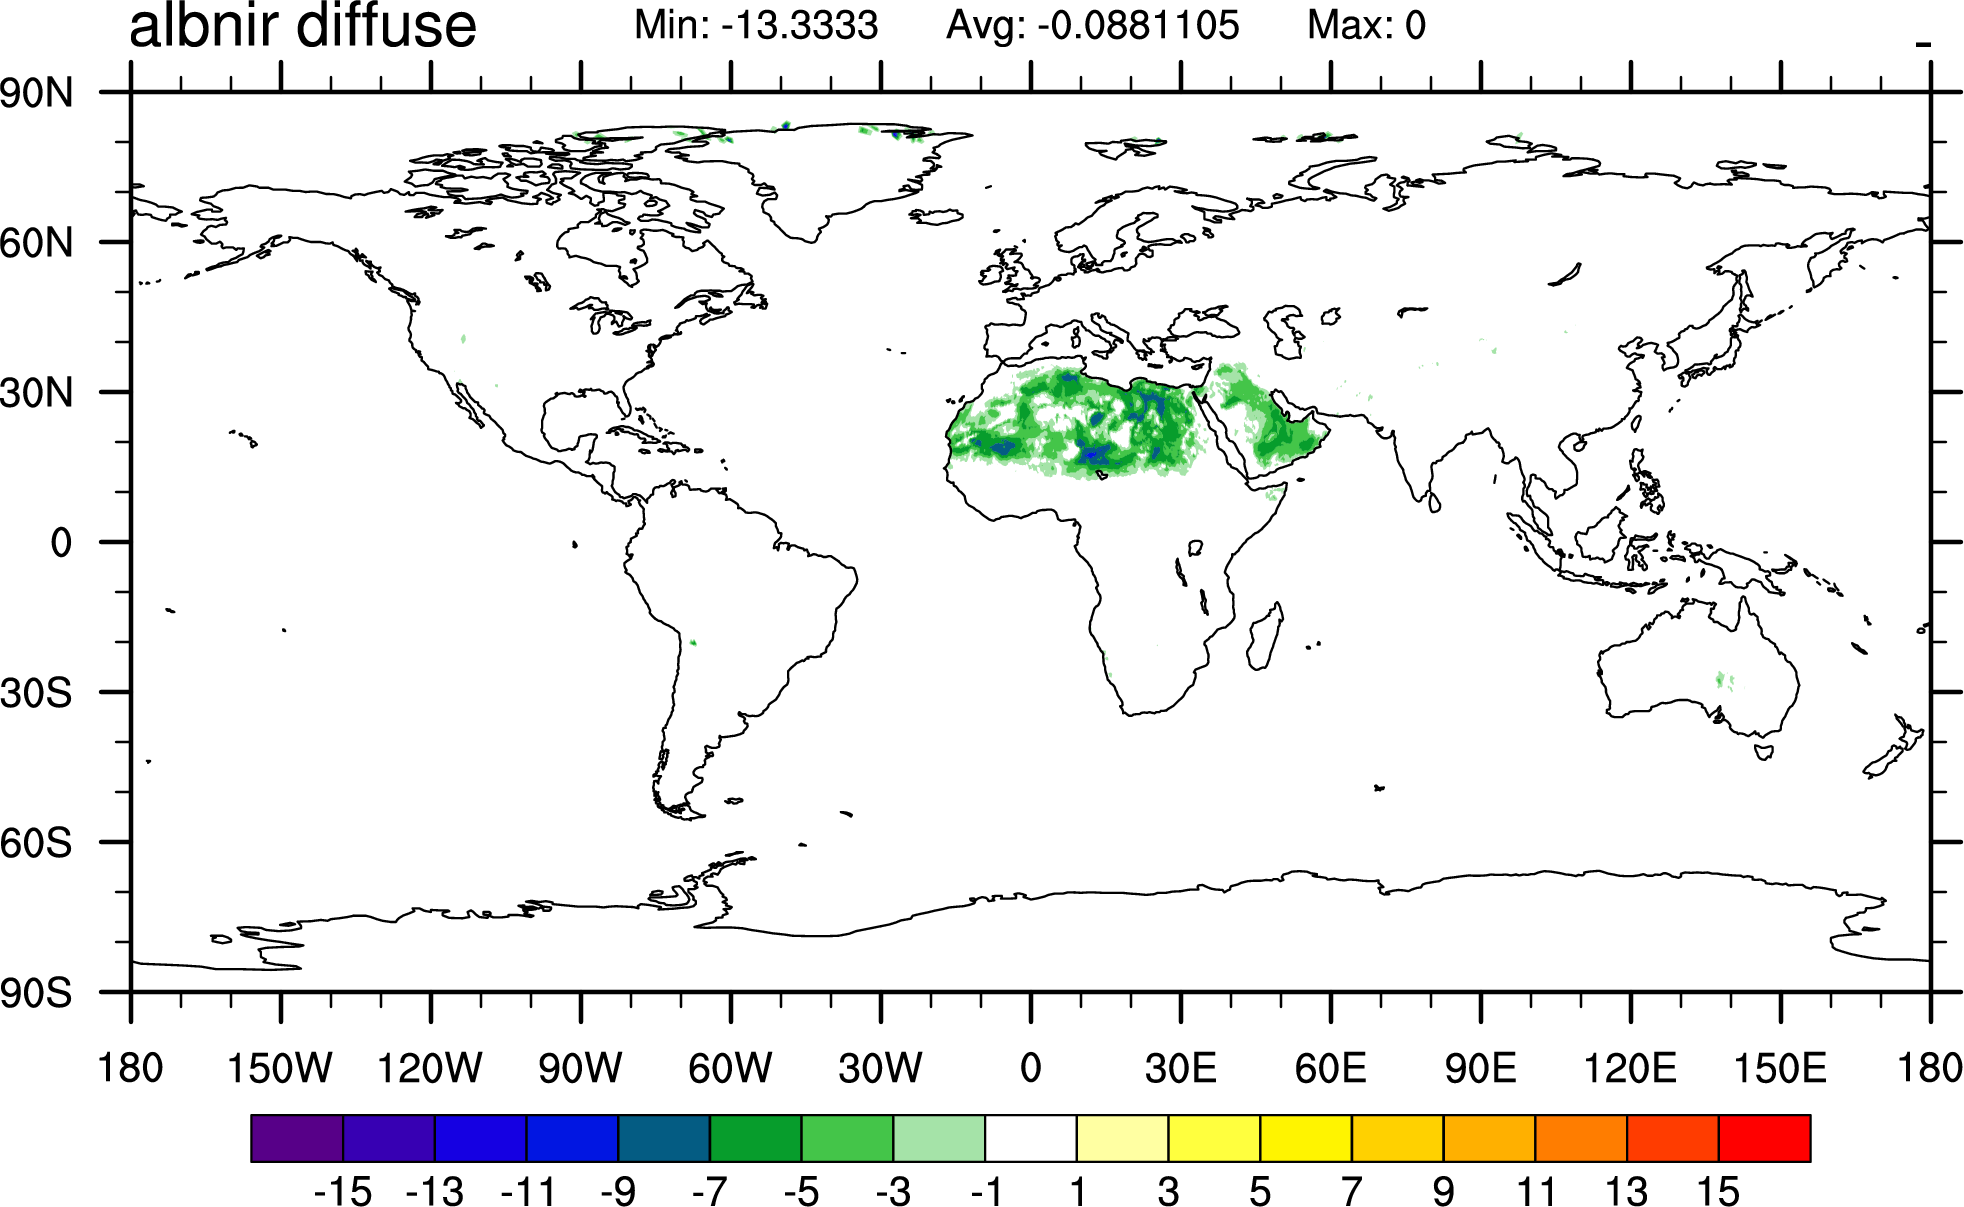
\includegraphics[width=7.7cm]{albnirdif_20120601_tuned-untuned.png}
  \end{minipage}
\end{minipage}
\caption{White sky (diffuse) albedo for near-infrared spectral bands (left) for the 1st June 2012 00UTC and its deviation from the original MODIS values (actual-original).}\label{fig_albnirdif}
\end{figure}



\subsection{Albedo for direct downward radiation (black sky)}
While surface albedo for the diffuse flux does not depend on the solar zenith angle (SZA) $\mu$, surface albedo for the direct flux does \citep{Yang:2008}. 
Up to ICON-NWP version $2.0.05$ the formula for taking into account the zenith angle dependency has been taken over from the Ritter-Geleyn radiation scheme. 
It is applied, irrespective of the underlying type of surface.
\begin{align}
  \alpha_{\mathrm{dir}}^{vis} = \frac{1.0 + 0.5\, \cos(\mu)  \left(\frac{1}{\alpha_{\mathrm{diff}}^{vis}}-1\right)}
                              {\left[1.0 + \cos(\mu)  \left(\frac{1}{\alpha_{\mathrm{diff}}^{vis}}-1\right)\right]^{2}} \label{eq_albvisdir}
\end{align}
\begin{align}
  \alpha_{\mathrm{dir}}^{nir} = \frac{1.0 + 0.5\, \cos(\mu)  \left(\frac{1}{\alpha_{\mathrm{diff}}^{nir}}-1\right)}
                              {\left[1.0 + \cos(\mu)  \left(\frac{1}{\alpha_{\mathrm{diff}}^{nir}}-1\right)\right]^{2}} \label{eq_albnirdir}
\end{align}
Note that the surface albedo for the direct flux is derived from the surface albedo for the diffuse flux, which is clearly an approximation. 
The parameterization is applied separately for the UV-visible and near-infrared spectral bands. An example for 1st June 2012 04UTC, 
based on the diffuse albedos shown in Figure \ref{fig_albvisdif} and \ref{fig_albnirdif} is given in Figure \ref{fig_albdir}. 
\begin{figure}[hbt]
\begin{minipage}[t]{\textwidth}
  \begin{minipage}[t]{0.498\textwidth}
    \center
    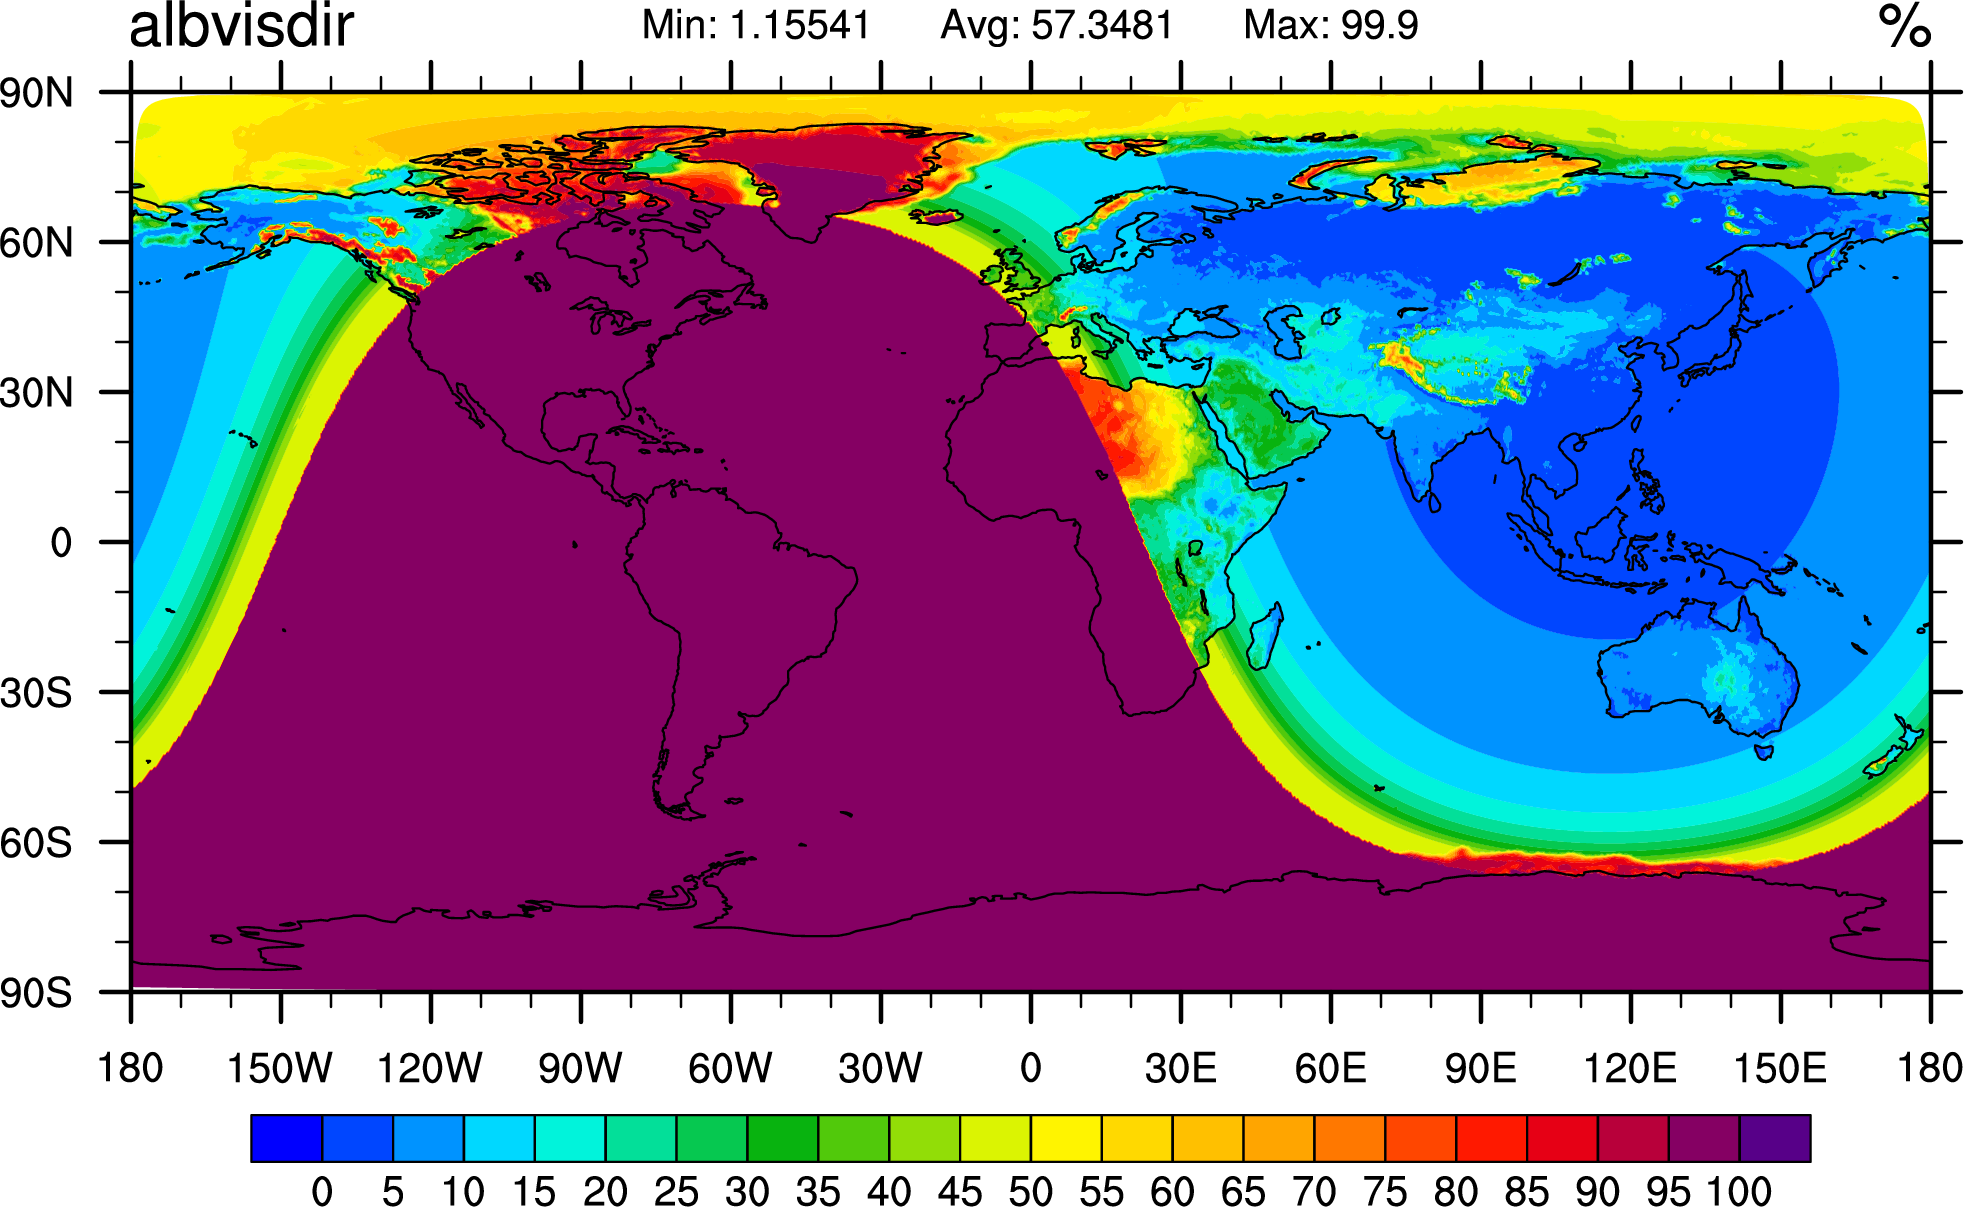
\includegraphics[width=8.1cm]{albvisdir_20120601_blacksky_ritter.png}
  \end{minipage}
  \begin{minipage}[t]{0.498\textwidth}
    \center
    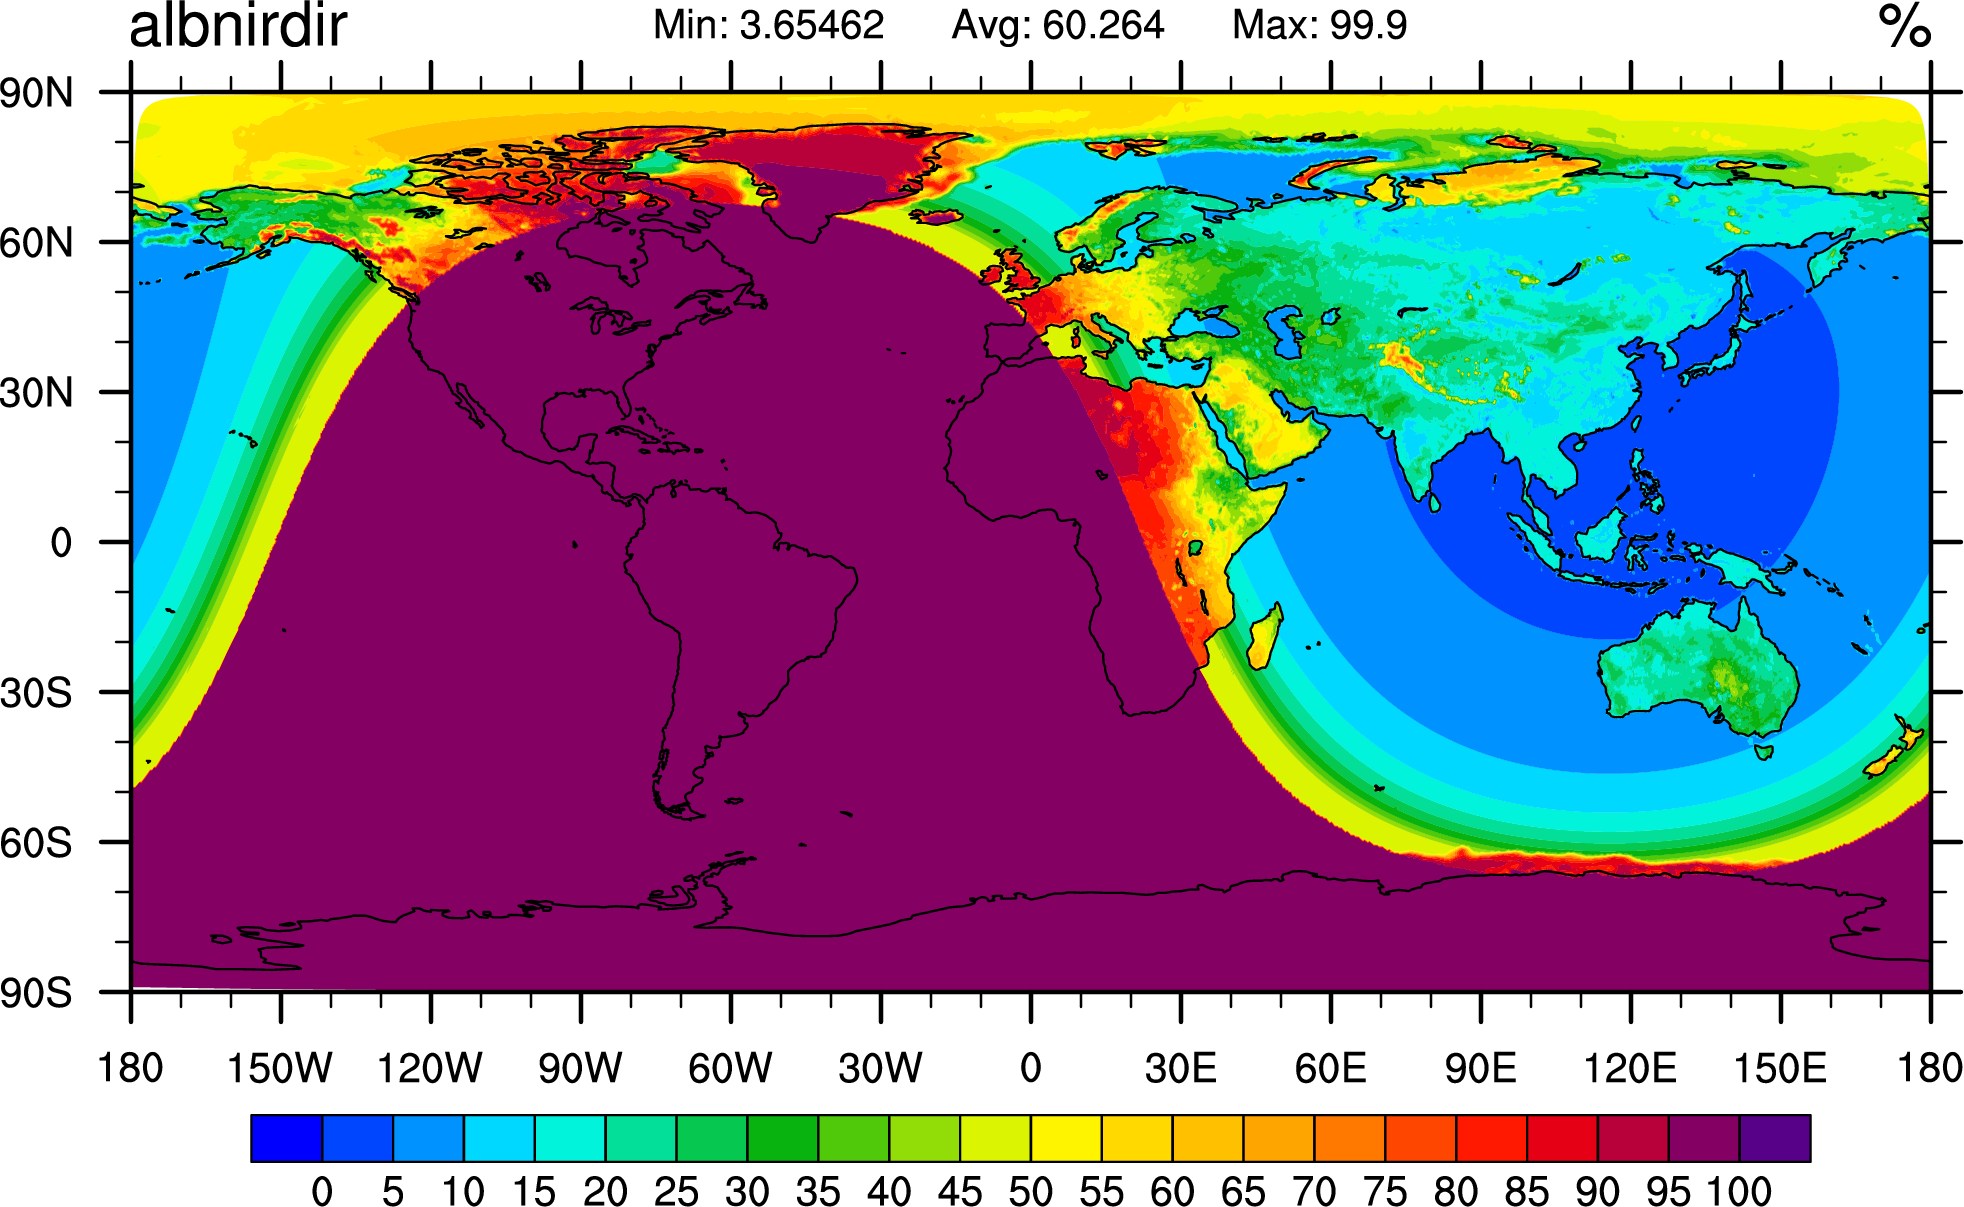
\includegraphics[width=8.2cm]{albnirdir_20120601_blacksky_ritter.png}
  \end{minipage}
\end{minipage}
\caption{Black sky (direct) albedo for UV-visible (left) and near-infrared (right) spectral bands for the 4th Jan 2012 04UTC.}\label{fig_albdir}
\end{figure}
The direct albedo seems to be overestimated significantly for large solar zenith angles.

From ICON-NWP version $2.0.06$ on, the black sky albedo is estimated as follows:
\begin{align}
 \alpha_{\mathrm{dir}} = \min\left[\alpha_{\mathrm{dir}},\alpha_{\mathrm{dir}}^{LIM}\right]
\end{align}
I.e.\ the black sky albedo computed according to equations \eqref{eq_albvisdir} and \eqref{eq_albnirdir} is not allowed to exceed the 
limit $\alpha_{\mathrm{dir}}^{LIM}$. The latter is defined as a weighted average of the unlimited black sky albedo $\alpha_{\mathrm{dir}}$ 
and the white sky albedo $\alpha_{\mathrm{diff}}$.
\begin{align}
 \alpha_{\mathrm{dir}}^{LIM} = \gamma \cdot \alpha_{\mathrm{diff}} + (1-\gamma)\cdot \alpha_{\mathrm{dir}}
\end{align}
The limit tends towards $\alpha_{\mathrm{diff}}$ the more rough the surface or oragraphy at the given grid point is. 
The weighting factor $\gamma$ is parameterized as a function of the SSO standard deviation $\sigma_{SSO}$ and 
the landuse class specific roughness length $z_{0}$. It is close to $0$ for landuse classes with 'smooth' vegetation/ orography 
and becomes $1$ for $z_{0}>0.15\,\mathrm{m}$ or $\sigma_{SSO}>150\,\mathrm{m}$.
\begin{align}
 \gamma &= \max\left[0.01\cdot (\sigma_{SSO}-50),10\cdot(z_{0}-0.05)\right]\\
 \gamma &= \min(1,\max(0,\gamma))
\end{align}
Thus, even for large SZA, the black sky albedo is not allowed to exceed the diffuse albedo, if the surface is 'rough'.



% \subsubsection{Sample plots}
% Figure \ref{fig_albvisdif} and \ref{fig_albnirdif} show the white sky surface albedo (UV-visible and near-infrared) for the 1st June 2012 00UTC as it is 
% operationally used by ICON for snow-free land points. Note that compared to the original MODIS data, the Saharan albedo has been slightly reduced in order 
% to compensate for a model cold bias in that region.
% 
% \begin{figure}[ht]
% \begin{minipage}[t]{\textwidth}
%   \begin{minipage}[t]{0.498\textwidth}
%     \center
%     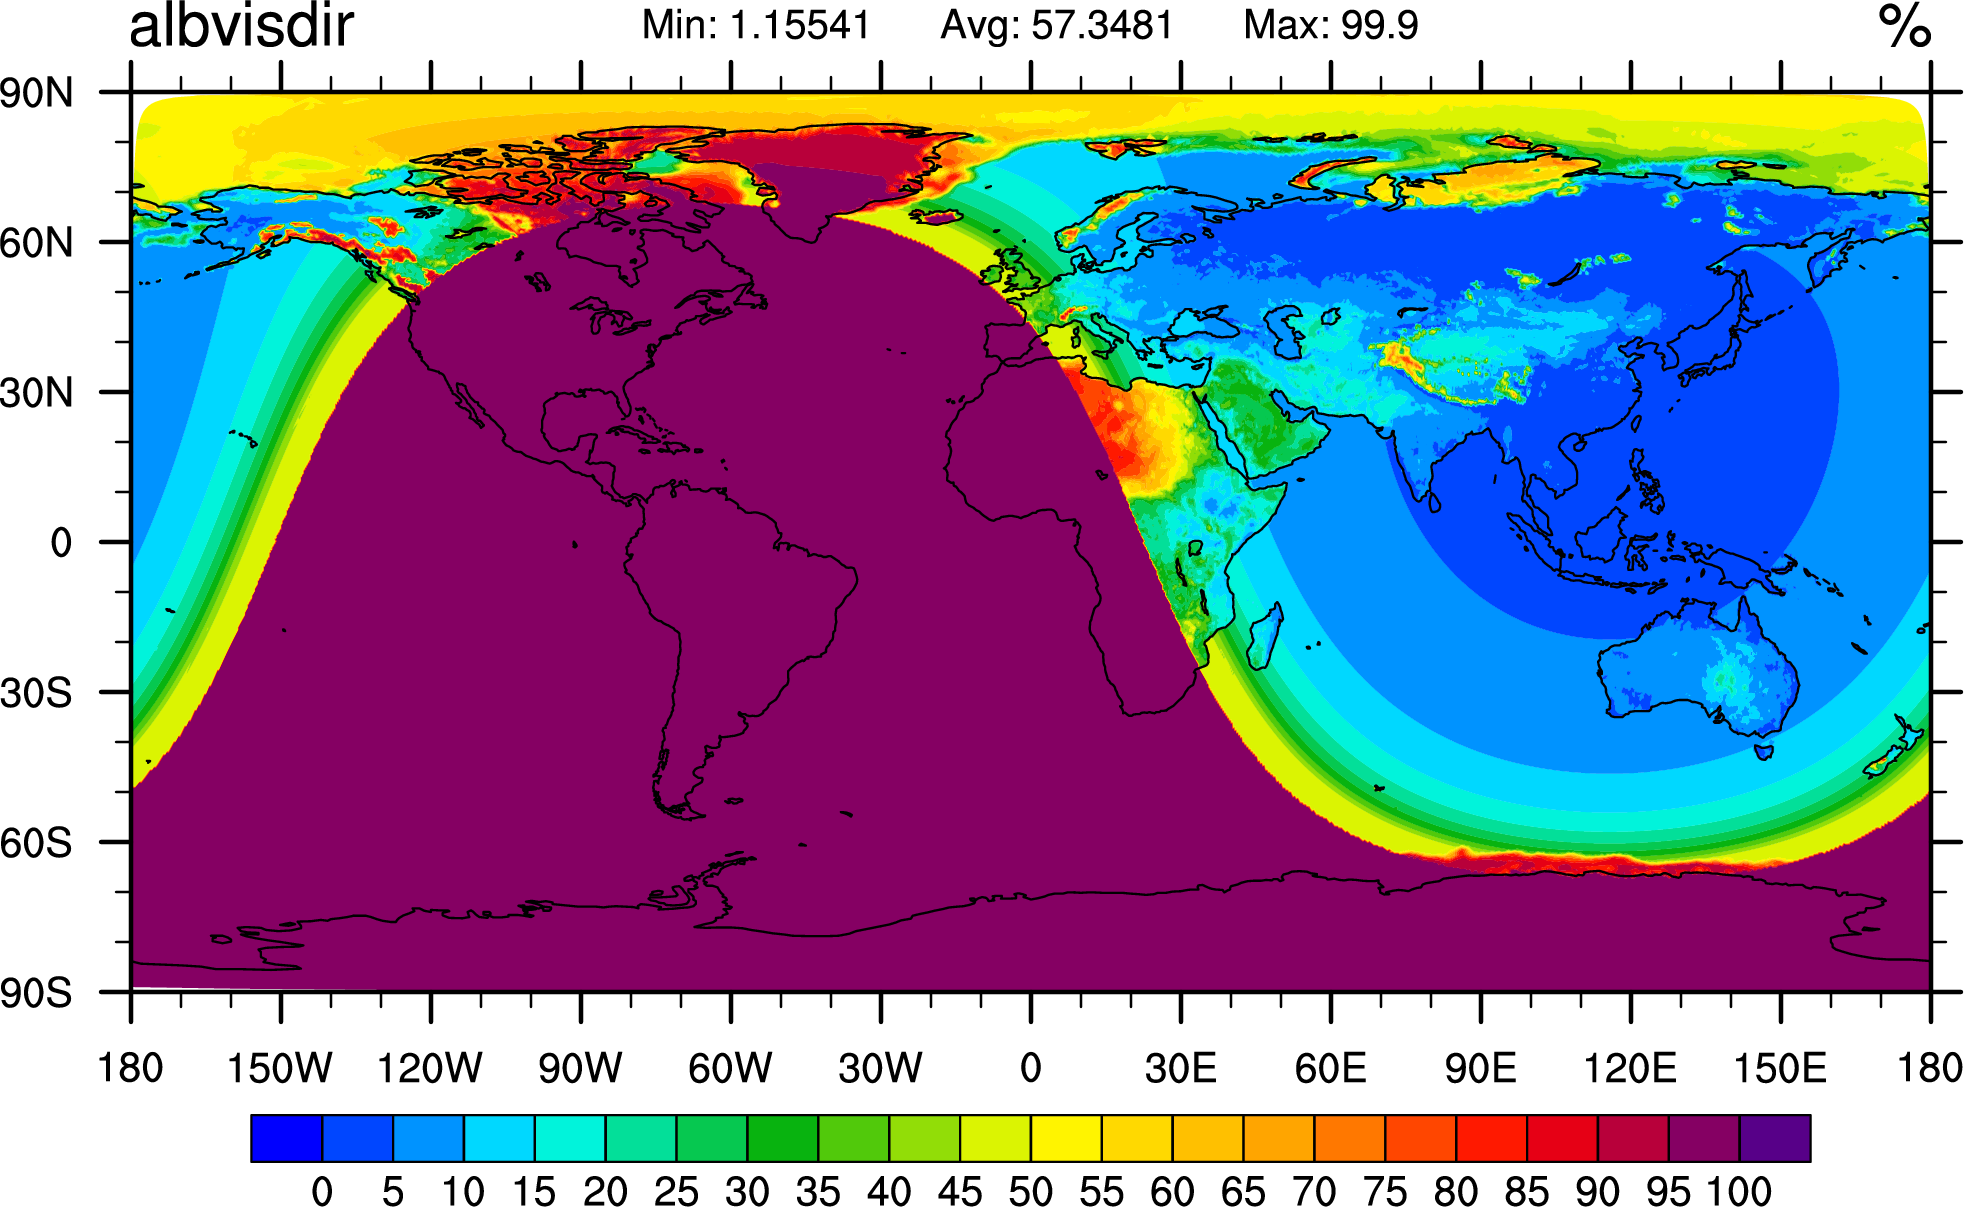
\includegraphics[width=8.1cm]{albvisdir_20120601_blacksky_ritter.png}
%   \end{minipage}
%   \begin{minipage}[t]{0.498\textwidth}
%     \center
%     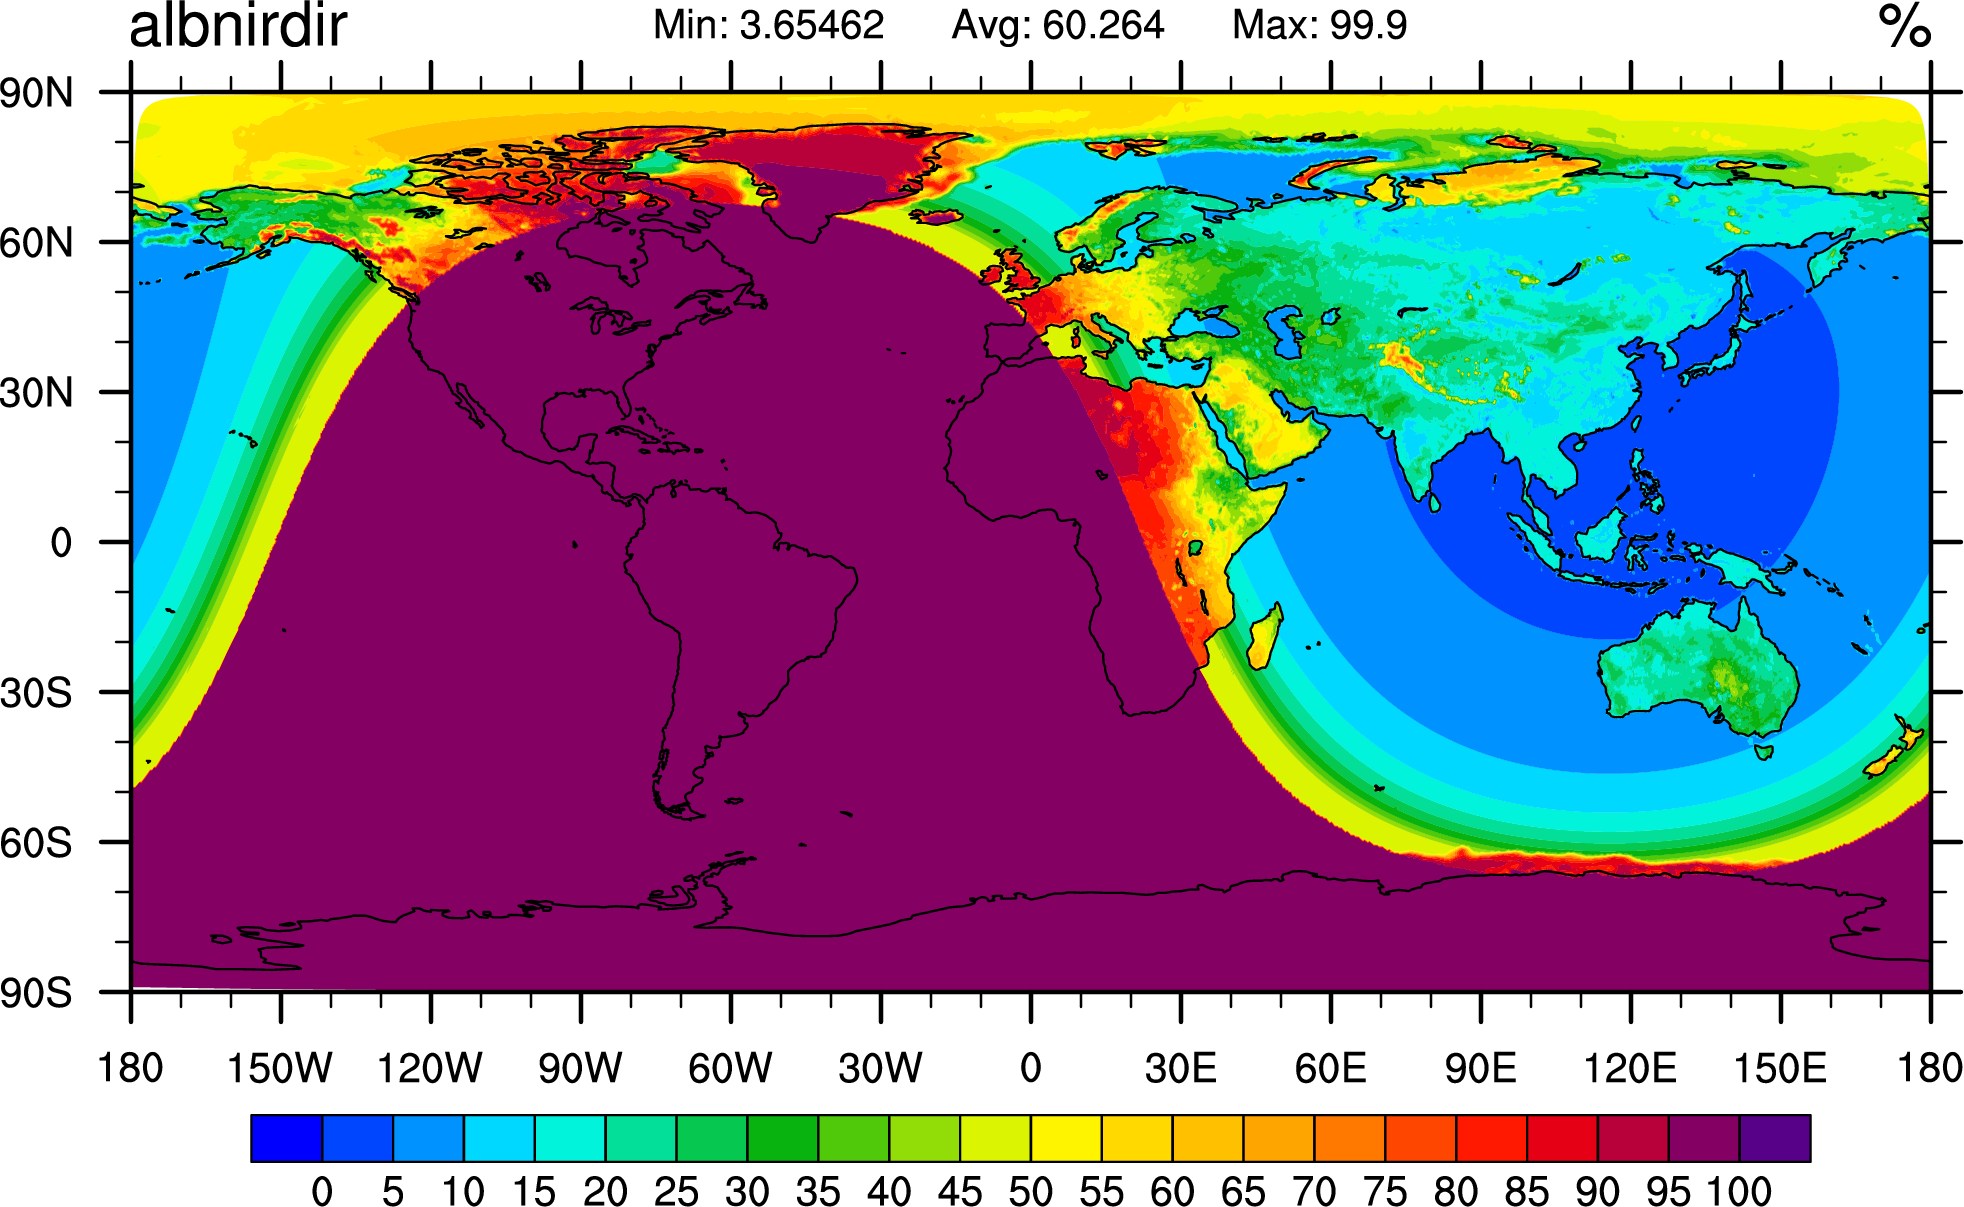
\includegraphics[width=8.2cm]{albnirdir_20120601_blacksky_ritter.png}
%   \end{minipage}
% \end{minipage}
% \caption{Black sky (direct) albedo for UV-visible (left) and near-infrared (right) spectral bands for the 4th Jan 2012 00UTC.}\label{fig_albdir}
% \end{figure}

%-------------------------------------------------------------------------

\bibliography {../references-icon-science}
\bibliographystyle {../wileyqj} %QJ


\end{document}
